% Pacotes
\documentclass[12pt]{article}
\usepackage{adjustbox}
\usepackage[utf8]{inputenc}
\usepackage{amsmath}
\usepackage{hyperref}
\usepackage{sbc-template}
\usepackage{fancyvrb}
\usepackage{amsfonts}
\usepackage{amsmath}
\usepackage{graphicx,url}


\sloppy

\title{Análise da Implementação de Algoritmo Genético\\para o Problema das P-Medianas}

\author{Ricardo Henrique Brunetto\inst{1}}


\address{Departamento de Informática -- Universidade Estadual de Maringá (UEM)\\
	Maringá -- PR -- Brasil
	\email{ra94182@uem.br}
}

\begin{document}

	\maketitle

  \section{Introdução}
	Este trabalho visa a apresentar uma implementação de um algoritmo genético para a resolução do problema das P-Medianas, descrito na seção seguinte. Tal implementação foi escrita em \textbf{Java}, por apresentar melhor manipulação de objetos em alto nível e maior quantidade de estruturas de dados e bibliotecas nativas. Considera-se de conhecimento do leitor os fundamentos da meta-heurística de Algoritmos Genéticos, que podem ser encontradas em \cite{alggen}.

	Além da implementação, serão brevemente analisados alguns casos de teste específicos que se encontram anexados, em arquivo, a relatório.

	O presente trabalho tem como objetivo obtenção de nota parcial na disciplina 6903 - Modelagem e Otimização Algorítmica no ano de 2017, ministrada pelo Prof. Dr. Ademir Constantino para a turma de Bacharelado em Ciência da Computação de 2015.

  \section{Descrição do Problema}

	Dado um grafo $G=(V, A)$, sendo que para cada vértices é associado um peso (demanda) e uma capacidade. O problema das $p$-Medianas tem como objetivo particionar o conjunto de vértices em p grupos. Para cada grupo de vértices deve ser associado a um vértice, denominado mediana. Os grupos devem ser formados de tal maneira que a soma das distâncias dos vértices do grupo à mediana seja mínima e a soma dos pesos (demandas) de todos os vértices de cada grupo não pode exceder a capacidade da mediana do grupo (incluindo a demanda do próprio vértice que é mediana).

  \section{Descrição do Algoritmo}
	Aqui será apresentada uma descrição de cada etapa do algoritmo. Serão expostas as decisões de projetos e escolhas de constantes para a implementação da meta-heurística.

	\subsection{Modelagem e Estrutura de Implementação}
	Modela-se o problema como um grafo, tal qual especificado. Para questões de implementação, constrói-se um \verb|Grafo|, que faz uso de um conjunto de vértices, implementado com \verb|HashSet|, uma vez que permite acesso direto (constante) através do índice do vértice. Considera-se um \verb|Vertice| um elemento com coordenadas $x$ e $y$ além de dois outros inteiros: $capacidade$ e $demanda$. Assim, um \verb|Vertice|, cujo conjunto compõe \verb|Grafo|, é um objeto cujos atributos provêm diretamente da entrada. Para facilitar a manipulação e identificação dos vértices (que podem ter mesmas coordenadas), adiciona-se um inteiro $id$ que será controlado pela Classe Principal.

	Contudo, percebe-se que é necessário guardar outras informações para que se possa realizar os cálculos pertinentes às funções de ajuste (abordadas a seguir). Para tanto, desenvolve-se uma Classe
	\verb|Solucao| que terá um $custo$, um agregado de \verb|VerticeSolucao| e um atributo do tipo \verb|Medianas|. Cada objeto da classe \verb|Solucao| representará \textbf{um indivíduo} da população.

	Quanto à classe \verb|VerticeSolucao|, a mesma é constituída pelos atributos de ponto-flutuante $difDistancia$ e $distancia$, que serão explanados futuramente; e pelos atributos inteiros $indexMediana$ e $indexCandidata$.

	Em relação à classe \verb|Medianas|, entende-se que será necessário dois agregados de inteiros: $indices$, para guardar o atributo $id$ de cada mediana, e $capacidades$, para guardar o atributo $capacidade$ de cada mediana, que varia conforme o cálculo da solução é realizado.

	Para executar um caso de teste, cria-se a classe \verb|RunTestes|, que será responsável por receber uma instância do problema, constituída pelos seguintes parâmetros:
	\begin{itemize}
		\item \textbf{tamanhoPopulacao}: tamanho da população que será considerada.
		\item \textbf{numeroGeracoes}: quantidade de iterações que o algoritmo executará.
		\item \textbf{numeroMedianas}: quantidade de medianas para a resolução do problema ($p$).
		\item \textbf{taxaDeElitismo}: porcentagem da população antiga a ser preservada.
		\item \textbf{taxaDeMutacao}: porcentagem dos indivíduos recém-gerados que serão mutados.
		\item \textbf{quantidadeReprodutores}: quantidade de indivíduos considerados para reprodução.
	\end{itemize}

	Com base em artigos da área, decidiu-se assumir os seguintes valores para alguns parâmetros:
	\begin{itemize}
		\item \textit{tamanhoPopulacao}: fixado em $30\%$ da quantidade de vértices do grafo de entrada.
		\item \textit{numeroGeracoes}: fixado em $30\%$ da quantidade de medianas multiplicado pela quantidade de vértices do grafo de entrada.
		\item \textit{taxaDeElitismo}: fixado em $10\%$.
		\item \textit{taxaDeMutacao}: fixado em $3\%$.
		\item \textit{quantidadeReprodutores}: fixado em $10$ indivíduos.
	\end{itemize}

	Além disso, todos os fatores randômicos executados pelo algoritmo são baseados na mesma semente ($SEED$, fixada com valor $5$).

	\subsection{População Inicial}
	A população inicial (função \verb|gerarPopulacaoInicial|) é gerada randomicamente. São gerados $tamanhoPopulacao$ soluções através da seleção aleatória de vértices para compor o conjunto das medianas. Após serem selecionados, analisa-se a validade da solução composta (se é possível que haja uma configuração de alocação para tais medianas) e então há o cálculo do custo.

	Cabe salientar que são consideradas apenas medianas distintas para compor as soluções iniciais.

	\subsection{Função de Ajuste (Fitness)}
	Para que seja permitido avaliar quantitativamente uma solução, propõe-se uma função de ajuste baseada em uma heurística. Em suma, a função que quantifica uma solução é:
	$$\sum_{i=0}^{n}d_i$$
	onde $d_i$ é a distância do vértice $i$ (atributo $distancia$) até a médiana que fora alocado.

	Em tal função, para cada vértice $v_i$ encontra-se $M_1$ e $M_2$, a mediana mais próxima e a segunda mediana mais próxima, respectivamente. Calcula-se, então, $d_{M_2} - d_{M_1}$, ou seja, a diferença entre as distâncias de $v_i$ para com suas duas medianas mais próximas. Esse valor permite estabelecer um \textbf{critério de prioridade} para alocação dos vértices. Assim, vértices com maior diferença entre as distâncias têm prioridade para serem alocados, o que justifica o uso de um \textit{Heap} Máximo. A motivação para tal decisão é que vértices que possuem uma discrepância maior entre suas medianas têm prioridade para serem alocados em suas medianas mais próximas pois, caso contrário, contribuirão com um valor maior para o somatório em da função (custo final da solução).

	Em termos de implementação, as diferenças entre as distâncias são calculadas e os vértices são incluídos em um \textit{Heap} (implementado pelo Java como \verb|PriorityQueue|) em ordem decrescente. A implementação deste procedimento está em \verb|calcularCusto|.

	\subsection{Seleção}
	Para seleção dos reprodutores, utiliza-se a \textbf{Seleção por Torneio}, realizando $quantidadeReprodutores$ torneios. Em cada torneio, seleciona-se aleatoriamente $quantidadeReprodutores$ indivíduos ainda não considerados e, dos selecionados, considera-se para reprodução o que apresenta melhor aptidão (valor de função \textit{fitness}).

	Dessa forma, garante-se certa heterogeneiadade ao compor o conjunto dos reprodutores, visto que permite considerar soluções com discrepância significativa de funções \textit{fitness} para cruzamento. Em termos de implementação, é realizado por \verb|selecionarReprodutores|.

	\subsection{Reprodução (Crossover)}
	Em relação à reprodução, utiliza-se a seguinte heurística: dados $2$ indivíduos do conjunto de reprodutores, cria-se um novo indivíduo que conterá em seu conjunto de medianas as medianas que seus pais têm em comum. As medianas faltam para completar as $numeroMedianas$ esperadas são sorteadas entre as medianas dos dois reprodutores que ainda não foram incluídas na solução.

	A justificativa para esta decisão é que os genes (medianas) em comum tendem a se perpetuar porque apresentam uma boa influência no valor da função objetivo (função \textit{fitness}). Dessa forma, incui-se tais genes no novo indivíduo gerado a fim de herdar tais características no custo final. Os demais genes são escolhidos aleatoriamente por questões de não ser considerado critério específico.

	A implementação deste procedimento é vista em \verb|cruzar|.

	\subsection{Busca Local} \label{bl}
	Primeiramente cabe salientar que foram desenvolvidos dois códigos: um com implementação da busca local e outro sem tal implementação. Doravante, o código que faz uso da busca local será denominado \textbf{Algoritmo Busca Local}, enquanto o código que não a utiliza será denominado \textbf{Algoritmo Clássico}.

	Em relação ao Algortimo Busca Local, implementa-se uma busca local que faz uso da estratégia de $best improvment$ para explorar a vizinhança. Dessa forma, aplica-se uma operação de movimentação a cada mediana da solução e considera-se a que mais oferece melhoria (redução de custo) em relação à original.

	A operação de movimentação, por sua vez, consiste em incrementar o $id$ da mediana (realizando verificação de não-continência), ou seja, escolher como mediana o próximo vértice da lista de entrada que ainda não está classificado como mediana.

	Dessa forma, inclui-se a própria solução na lista da vizinhança e retorna-se a que possui melhor custo associado. A implementação deste procedimento é vista em \verb|buscaLocal| no código Algoritmo Busca local.

	\subsection{Mutação}
	Em relação à mutação, é aplicado uma operação de mutação a $taxaDeMutacao$ da população \textbf{recém-gerada}. Ou seja, não é aplicada mutação para os indivíduos reprodutores ou outros já contidos na solução.

	A operação de mutação consiste em sortear uma mediana do conjunto do indivíduo recém-gerado e substituí-la por outra mediana, também escolhida aleatoriamente, que ainda não está no conjunto. Como a proposta da mutação é executar uma ligeira mudança (alteração elementar) e arbitrária na solução, considera-se suficiente alterar uma única mediana.

	A implementação deste procedimento está em \verb|aplicarMutacao|.

	\subsection{Atualização da População}
	Para atualização da população, considera-se a estratégia de \textbf{elitismo}, onde se mantém $taxaDeElitismo$ da população antiga (que têm melhor aptidão), e insere-se a população recém-gerada.

	Nesse quesito, houve cuidado apenas para não extrapolar ou não atingir o tamanho da população, que se mantém constante durante as gerações (iterações) do algoritmo, com o valor de $tamanhoPopulacao$.

	\section{Testes e Resultados}
	Conforme descrito na seção \ref{bl}, são consideradas duas vertentes do algoritmo: com e sem busca local após a geração de um novo indivíduo. Foram executados $6$ casos de teste para cada uma das duas implementações.

	Para cada um dos casos de teste, considera-se a melhor solução (de melhor custo) encontrada para calcular os parâmetros solicitados.

	A tabela \ref{tab:graf1} mostra as informações a respeito dos casos de teste.
	\begin{table}[]
\centering
\label{tab:graf1}
\begin{tabular}{ccclll}
\hline
\multicolumn{1}{|c|}{\textit{Caso}} & \multicolumn{1}{c|}{\textit{MS}} & \multicolumn{1}{c|}{\textit{Alg}} & \multicolumn{1}{l|}{$GAP_1\%$} & \multicolumn{1}{l|}{\textit{Alg\_bl}} & \multicolumn{1}{l|}{$GAP_2\%$} \\ \hline
SJC1                                & 17288,99                         & 17523,72                          & 1,35                           & 17523,72                              & 1,35                           \\
SJC2                                & 33270,94                         & 36509,90                          & 9,73                           & 36509,90                              & 9,73                           \\
SJC3a                               & 45335,16                         & 47327,86                          & 4,39                           & 47327,86                              & 4,39                           \\
\multicolumn{1}{l}{SJC3b}           & \multicolumn{1}{l}{40635,90}     & \multicolumn{1}{l}{41886,10}      & 3,07                           & 41886,10                              & 3,07                           \\
\multicolumn{1}{l}{SJC4a}           & \multicolumn{1}{l}{61925,51}     & \multicolumn{1}{l}{62276,45}      & 0,56                           & 62276,45                              & 0,56                           \\
\multicolumn{1}{l}{SJC4b}           & \multicolumn{1}{l}{52458,02}     & \multicolumn{1}{l}{53604,41}      & 2,18                           & 53604,41                              & 2,18
\end{tabular}
\caption{Informações dos Casos de Teste}
\end{table}

	\paragraph{Convergência com Algoritmo Clássico}
	Nesse caso, é apresentado o gráfico de convergência na Figura \ref{fig:graf1}.
	\begin{figure}[h]
	 	\centering
	 	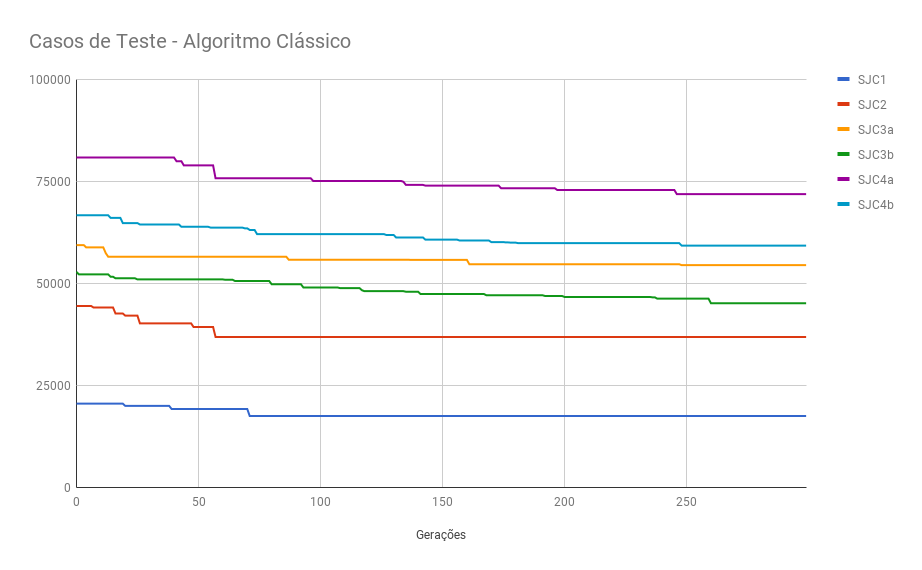
\includegraphics[scale = 0.5]{graf1.png}
		\label{fig:graf1}
	 	\caption{Convergência com Algoritmo Clássico}
	 \end{figure}

	 É cabível salientar que não há alteração expressiva visível nas linhas do gráfico devido à discrepância da escala de valores entre os casos de teste.

	\paragraph{Convergência com Algoritmo Busca Local}
	Nesse caso, é apresentado o gráfico de convergência na Figura \ref{fig:graf2}.
	\begin{figure}[h]
		\centering
		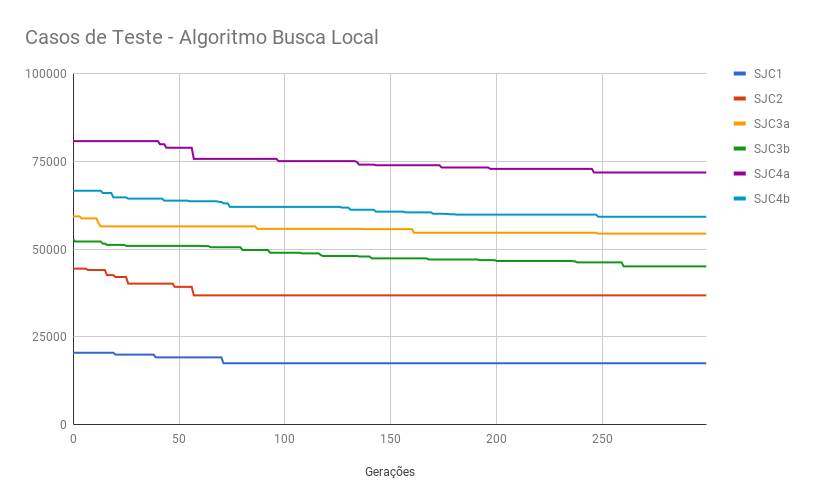
\includegraphics[scale = 0.5]{graf2.png}
		\label{fig:graf2}
		\caption{Convergência com Algoritmo Busca Local}
	 \end{figure}

	É cabível salientar que não há alteração expressiva visível nas linhas do gráfico devido à discrepância da escala de valores entre os casos de teste.

	\section{Conclusão}
	Em suma, a busca local proporciona convergência e maior precisão dos resultados, visto que analisa a vizinhança de cada indivíduo antes de inserí-lo cegamente na população. Dessa forma, há inclusão do ótimo local de cada indivíduo e, portanto, a composição de uma população com soluções ótimas em suas respectivas vizinhanças.

	Contudo, o uso da Busca Local consome uma carga muito maior de processamento para instâncias maiores e maior tempo computacional. Além disso, neste caso não houve expressividade no uso da busca local. Provavelmente se deve ao tipo de exploração da vizinhança. É provável que com outras operações de movimentação haja diferenças significativas.

	\bibliographystyle{sbc}
	\bibliography{references}

\end{document}
